\documentclass[11pt]{article}
\usepackage[margin=1in]{geometry}
\usepackage{amsmath,amssymb,booktabs,graphicx}
\graphicspath{{../results/}}
\newcommand{\Yhat}{\widehat Y}
\newcommand{\DP}{\Delta_{\mathrm{DP}}}

\title{ECE 750T Assignment 1}
\author{Yehia Fahmy\\Student ID: [placeholder]}
\date{}

\begin{document}
\maketitle

\section*{Question 1}

\subsection*{Q1.1}
On the training set, ranking by absolute Pearson correlation and breaking ties by column index gives the following signed correlations.

\begin{center}
\small
\begin{tabular}{lr}
\toprule
Feature correlated with $Y$ & Correlation \\
\midrule
\texttt{marital-status\_Married-civ-spouse} & 0.4447 \\
\texttt{relationship\_Husband} & 0.4010 \\
\texttt{education\_num} & 0.3352 \\
\texttt{marital-status\_Never-married} & $-0.3184$ \\
\texttt{age\_u30} & $-0.2381$ \\
\texttt{hours-per-week} & 0.2297 \\
\texttt{relationship\_Own-child} & $-0.2285$ \\
\texttt{capital-gain} & 0.2233 \\
\texttt{occupation\_Exec-managerial} & 0.2149 \\
\texttt{relationship\_Not-in-family} & $-0.1885$ \\
\bottomrule
\end{tabular}
\end{center}

\begin{center}
\small
\begin{tabular}{lr}
\toprule
Feature correlated with $A$ & Correlation \\
\midrule
\texttt{relationship\_Husband} & 0.5801 \\
\texttt{marital-status\_Married-civ-spouse} & 0.4318 \\
\texttt{relationship\_Unmarried} & $-0.3213$ \\
\texttt{relationship\_Wife} & $-0.3193$ \\
\texttt{occupation\_Adm-clerical} & $-0.2631$ \\
\texttt{hours-per-week} & 0.2293 \\
\texttt{marital-status\_Divorced} & $-0.2286$ \\
\texttt{occupation\_Craft-repair} & 0.2231 \\
\texttt{marital-status\_Widowed} & $-0.1885$ \\
\texttt{marital-status\_Never-married} & $-0.1714$ \\
\bottomrule
\end{tabular}
\end{center}

\subsection*{Q1.2}
The supplied classifier, trained with $\alpha=0$, has test accuracy $0.8557$, reweighted accuracy $0.8738$, and $\DP=0.1707$. The positive-prediction rate is $0.0880$ for $A=0$ (Female) and $0.2587$ for $A=1$ (Male), so Male has the higher average prediction.

\subsection*{Q1.3}
The three strongest test-set correlations with $\Yhat$, again ranked by absolute correlation, are:

\begin{center}
\small
\begin{tabular}{llr}
\toprule
Subset & Feature & Correlation \\
\midrule
All & \texttt{marital-status\_Married-civ-spouse} & 0.4686 \\
All & \texttt{education\_num} & 0.4336 \\
All & \texttt{relationship\_Husband} & 0.4177 \\
$A=0$ & \texttt{relationship\_Wife} & 0.5620 \\
$A=0$ & \texttt{marital-status\_Married-civ-spouse} & 0.5273 \\
$A=0$ & \texttt{capital-gain} & 0.2987 \\
$A=1$ & \texttt{education\_num} & 0.4913 \\
$A=1$ & \texttt{relationship\_Husband} & 0.4151 \\
$A=1$ & \texttt{marital-status\_Married-civ-spouse} & 0.4105 \\
\bottomrule
\end{tabular}
\end{center}

\subsection*{Q1.4}
\paragraph{(a)}
For a batch containing both groups, let $r_i\in(0,1)$ be the sigmoid score and $B_a=\{i:A_i=a\}$. The penalty is
\[
L_{\mathrm{DP}}
=
\left(
\frac1{|B_0|}\sum_{i\in B_0} r_i
-
\frac1{|B_1|}\sum_{i\in B_1} r_i
\right)^2.
\]
The minimized objective is binary cross-entropy plus $\alpha L_{\mathrm{DP}}$. Each score is a composition of smooth network operations and the sigmoid, both group means are linear in those scores, and $z\mapsto z^2$ is smooth. Thus $L_{\mathrm{DP}}$ has a gradient with respect to the network parameters. A thresholded prediction would be constant almost everywhere and would not provide this gradient. Batches missing either group use classification loss alone.

\paragraph{(b)}
Training-set sweeps showed that $\alpha=0.1$ barely reduced the DP gap, while $\alpha\in\{300,1000\}$ pushed both groups' positive rates to approximately zero. The useful comparison range, including the baseline, is therefore
\[
\alpha\in\{0,1,3,10,30,100\}.
\]
All runs use seed 0 and the supplied training settings. The test curves are shown below; tabulated values are rounded to four decimals.

\begin{center}
\begin{tabular}{rrrr}
\toprule
$\alpha$ & Accuracy & Reweighted accuracy & $\DP$ \\
\midrule
0 & 0.8557 & 0.8738 & 0.1707 \\
1 & 0.8509 & 0.8678 & 0.0958 \\
3 & 0.8442 & 0.8599 & 0.0514 \\
10 & 0.8389 & 0.8554 & 0.0211 \\
30 & 0.8325 & 0.8516 & 0.0012 \\
100 & 0.8018 & 0.8312 & 0.0040 \\
\bottomrule
\end{tabular}
\end{center}

\begin{center}
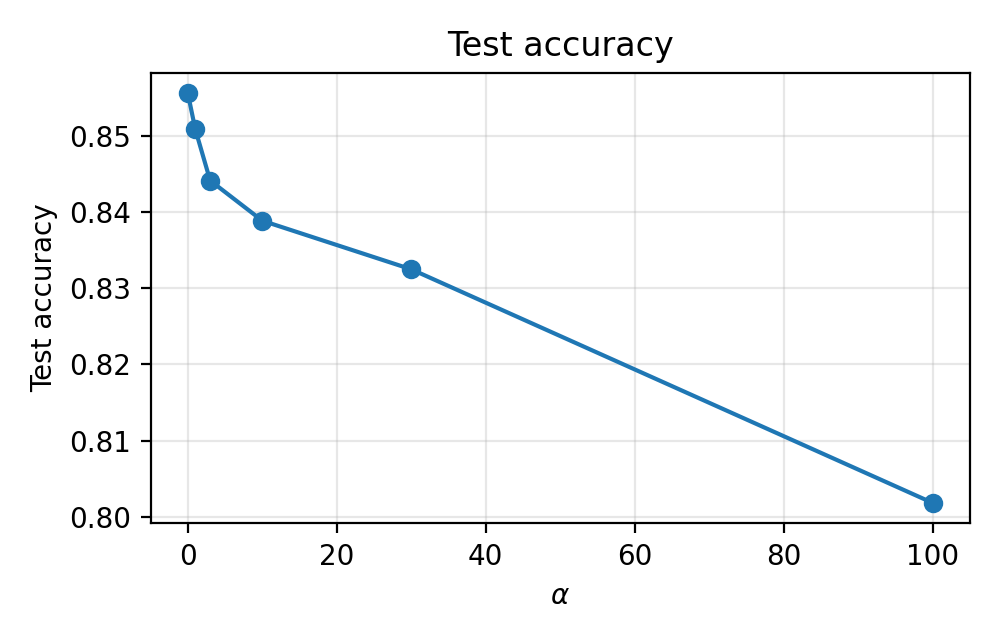
\includegraphics[width=0.62\textwidth]{q14_accuracy.png}\\[0.5em]
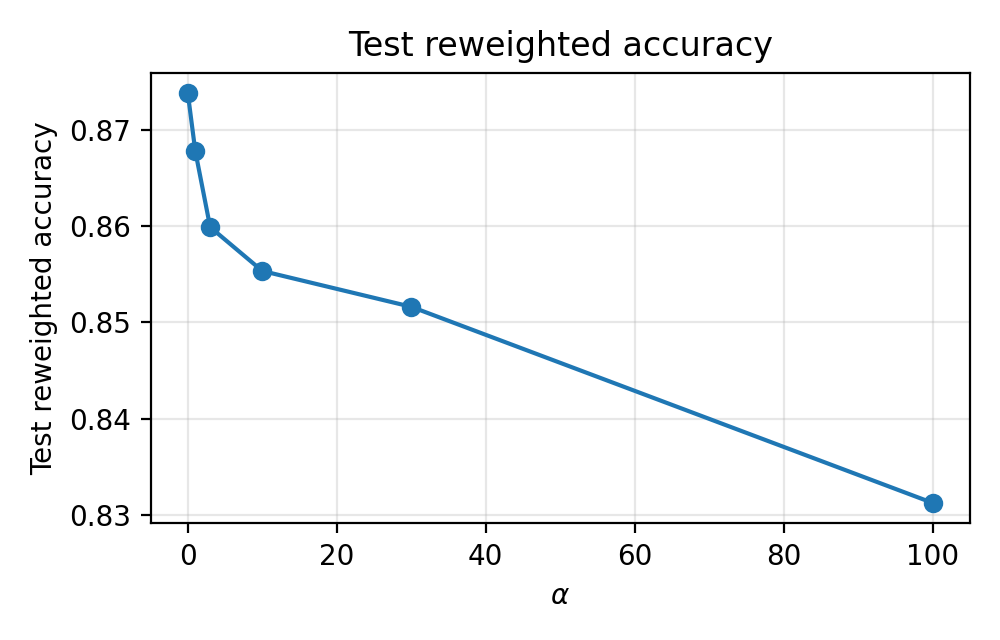
\includegraphics[width=0.62\textwidth]{q14_rw_accuracy.png}\\[0.5em]
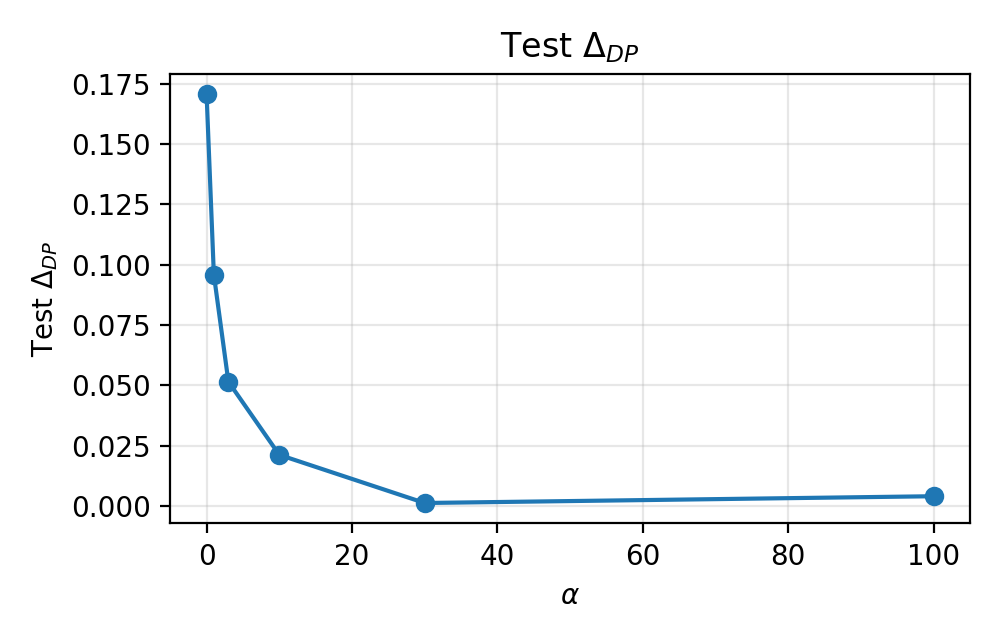
\includegraphics[width=0.62\textwidth]{q14_dp_gap.png}
\end{center}

Increasing $\alpha$ from 0 to 30 reduces test $\DP$ from 0.1707 to 0.0012 while accuracy falls by about 0.023 and reweighted accuracy by about 0.022. At $\alpha=100$, the gap remains near zero, but accuracy falls further to 0.8018 because positive predictions become rare in both groups. The DP curve is not monotone: the gap is 0.0012 at $\alpha=30$ and 0.0040 at $\alpha=100$.

\section*{Question 2}

\subsection*{Q2.1}
Let $X,R$ be independent Bernoulli$(1/2)$ variables and set $Y=X+R\pmod 2$. The joint distribution has four atoms,
\[
(X,R,Y)\in\{(0,0,0),(0,1,1),(1,0,1),(1,1,0)\},
\]
each with probability $1/4$.

For every $x,r\in\{0,1\}$, $P(X=x,R=r)=1/4=P(X=x)P(R=r)$, so $X\perp R$.

Now $P(Y=0)=1/2$, and the conditional outcomes are $(X,R)=(0,0)$ and $(1,1)$, each with probability $1/2$. Hence
\[
P(X=1,R=1\mid Y=0)=\frac12,
\]
whereas
\[
P(X=1\mid Y=0)P(R=1\mid Y=0)=\frac12\cdot\frac12=\frac14.
\]
The two quantities differ, so $X\not\perp R\mid Y$.

\subsection*{Q2.2}
Let $P(A=0)=P(A=1)=1/2$,
\begin{align*}
P(Y=1\mid A=0)&=\frac12,&
P(Y=2\mid A=0)&=\frac14,&
P(Y=3\mid A=0)&=\frac14,\\
P(Y=1\mid A=1)&=\frac14,&
P(Y=2\mid A=1)&=\frac14,&
P(Y=3\mid A=1)&=\frac12,
\end{align*}
and let $R=\mathbf 1\{Y\neq 2\}$. The resulting joint atoms are
\begin{center}
\begin{tabular}{ccccccc}
\toprule
$(A,Y,R)$ & $(0,1,1)$ & $(0,2,0)$ & $(0,3,1)$ & $(1,1,1)$ & $(1,2,0)$ & $(1,3,1)$ \\
Probability & $1/4$ & $1/8$ & $1/8$ & $1/8$ & $1/8$ & $1/4$ \\
\bottomrule
\end{tabular}
\end{center}
Both groups and all three target values have positive probability. Since $P(Y=1\mid A=0)=1/2$ but $P(Y=1)=3/8$, it follows that $A\not\perp Y$.

Given either value of $A$, $P(R=1\mid A)=3/4=P(R=1)$, so $R\perp A$. Given any value of $Y$, $R$ is deterministic and therefore independent of $A$. Thus $R\perp A\mid Y$. Independence and separation hold simultaneously even though $A$ and $Y$ are dependent.

\subsection*{Q2.3}
Let $p_a=P(g(X)=1\mid A=a)$ and $\delta=p_1-p_0$, so $\DP(g)=|\delta|$. Define $h(X)=g(X)$ when $\delta\ge 0$, and $h(X)=1-g(X)$ when $\delta<0$. In either case $h$ is a function of $X$.

If $\delta\ge 0$, then
\begin{align*}
\mathrm{RWAcc}_A(h)
&=\frac12\bigl(P(h=0\mid A=0)+P(h=1\mid A=1)\bigr)\\
&=\frac12\bigl(1-p_0+p_1\bigr)
=\frac12+\frac12\delta
=\frac12+\frac12\DP(g).
\end{align*}
If $\delta<0$, then
\begin{align*}
\mathrm{RWAcc}_A(h)
&=\frac12\bigl(P(g=1\mid A=0)+1-P(g=1\mid A=1)\bigr)\\
&=\frac12+\frac12(p_0-p_1)
=\frac12+\frac12\DP(g).
\end{align*}
Therefore $\mathrm{RWAcc}_A(h)\ge \tfrac12\DP(g)+\tfrac12$.

\section*{Assistance disclosure}
Cursor, a generative-AI coding assistant, was used to implement the required functions and analysis script, run the supplied training and evaluation workflow, generate the figures, and draft this write-up. The code, metric checks, numerical results, and proofs were reviewed against the assignment definitions.

\end{document}
